\documentclass[xcolor=dvipsnames]{beamer}
\usepackage[utf8]{inputenc}
\usepackage[IL2]{fontenc}
\usepackage[czech]{babel}
\usepackage{float}
\usepackage{listings}
\usepackage{amssymb}
\usepackage{amsmath}
\usepackage{mathtools}
\usepackage{url}
\usepackage{graphicx}
%\useoutertheme[subsection=false]{smoothbars}
\usetheme{Madrid}
\usecolortheme[named=OliveGreen]{structure}
\title{Tvorba agentových modelů}
\author{Marek Bryša}
\institute
{
Masarykova Univerzita\\
Přírodovědecká fakulta\\
Ústav matematiky a statistiky
}
\date{Obhajoba bakalářské práce}

\begin{document}
  \frame{\titlepage}
  \begin{frame}
    \frametitle{Cíl práce}
    Analýza síťového marketingu z ekonomického pohledu\\
  \end{frame}
  \begin{frame}
    \frametitle{Síťový marketing}
    Systém, kde se samotní spotřebitelé mohou stát za určitých podmínek prodejci
a distribuovat výrobky.\\
    K tomu a zejména k přivedení dalších lidí se je provozovatel prodejní sítě snaží finančně motivovat.\\
    Ušetří naopak drtivou většinu nákladů na vybudování kamenných provozoven. 
  \end{frame}
  \begin{frame}
    \frametitle{Dílčí cíle}
    \begin{itemize}
      \item Vznik prodejní sítě a průběh jejího šíření
      \item Zkoumání výsledné struktury
      \item Odvození příjmových a nákladových funkcí provozovatele
      \item Doporučení vedoucí k maximalizaci jeho zisku
    \end{itemize}
  \end{frame}
  \begin{frame}
    \frametitle{Metoda}
    \begin{enumerate}
      \item Zaměření na konkrétní fungujíci systém -- firma Oriflame (kosmetické výrobky)
      \item Vytvoření počítačového multiagentového modelu
      \item Provedení simulací a experimentů na něm
      \item Analýza dat pomocí ekonometrických a statistických nástrojů

    \end{enumerate}

  \end{frame}
  \begin{frame}
    \frametitle{Oriflame}
    Možnost výdelku pro prodejce (člena Oriflame):
    \begin{itemize}
      \item Marže z přímého prodeje -- od Oriflame koupím za 75 Kč, prodám známému za 100 Kč
      \item Přivedení dalších lidí k prodejní síti -- dostanu podle určitého schematu procenta z prodeje lídí, které jsem přivedl, které oni přivedli, atd.
    \end{itemize}
    Náklady prodejce:
    \begin{itemize}
      \item Obětovaný čas
      \item Případný pravidelný fixní poplatek -- Oriflame jej nevybíra, zkoumání jeho vlivu je však zajímavé
    \end{itemize} 
  \end{frame}
  \begin{frame}
    \frametitle{Hlavní výsledky}
    \framesubtitle{Generování grafu sociálních vazeb}
    \begin{center}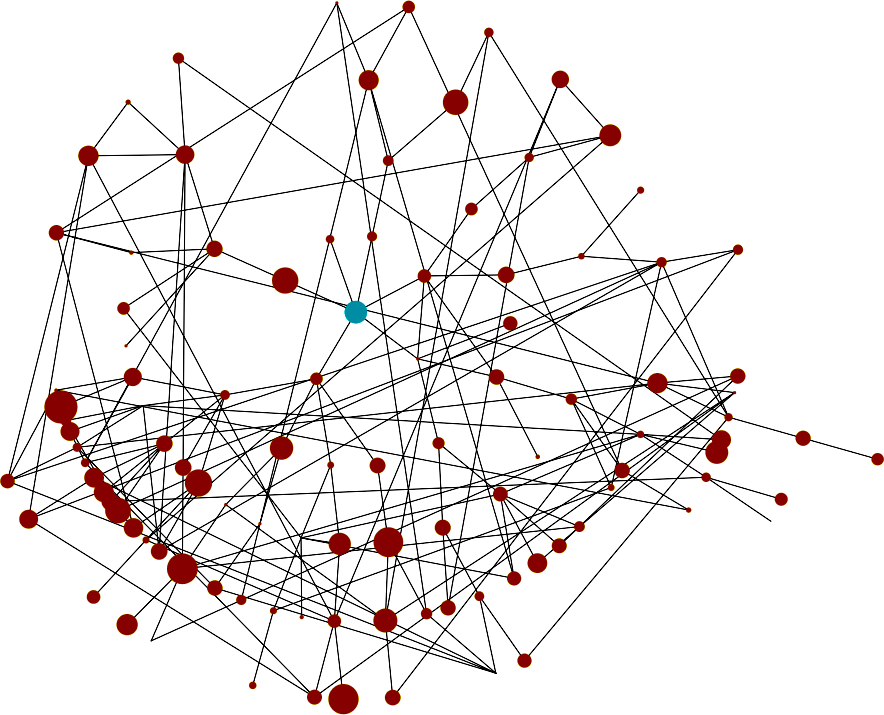
\includegraphics[width=0.6\textwidth]{oriflame7_view1.png}\end{center}
  \end{frame}
  \begin{frame}
    \frametitle{Hlavní výsledky}
    \framesubtitle{Průběh šíření}
    \begin{enumerate}
      \item Bouřlivý nárůst počtu prodejců
      \item Postupný pokles
      \item Stabilizace na přibližne čtvrtině celkového počtu osob v modelu
    \end{enumerate}
    \begin{center}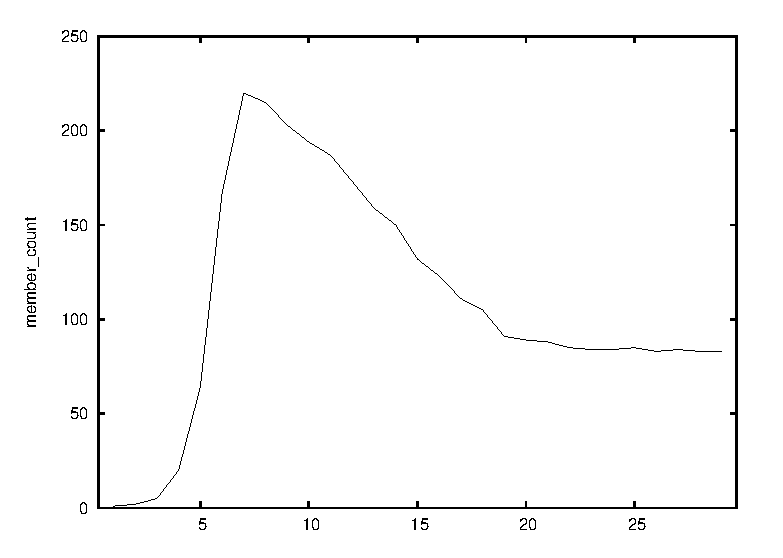
\includegraphics[width=0.6\textwidth]{member_count.eps}\end{center}
  \end{frame}
  \begin{frame}
    \frametitle{Hlavní výsledky}
    Vlastnosti prodejců:
    \begin{itemize}
      \item Nadprůměrný počet přátel
      \item Podprůměrné alternativní náklady $\Rightarrow$ stačí nižší výdělek, aby se členství v prodejní sítí dané osobě vyplatilo
    \end{itemize}
    Identifikace tzv. slabých článků -- osob bránících šíření prodejní sítě:
    \begin{itemize}
      \item Podprůměrný počet přátel $\Rightarrow$ nízký zisk z prodeje 
      \item Nadprůměrné alternativní náklady
    \end{itemize}
  \end{frame}
  \begin{frame}
    \frametitle{Hlavní výsledky}
    \framesubtitle{Analýza příjmů a nákladů provozovatele}
    Pro danou sociální síť jsou příjmy funkcí prodejní marže prodejců a pravidelně vybíraného poplatku -- tyto parametry mají významný na počet osob, kterým se vyplatí být prodejci.\\
    Variabilní náklady jsou funkcí stejných parametrů a navíc výrobních nákladů, které ovšem nejsou pro Oriflame známy a je tak možno je v modelu měnit.\\
    Fixní náklady nejsou uvažovány, neboť nemají vliv na polohu maxima zisku.\\
  \end{frame}
  \begin{frame}
    \frametitle{Hlavní výsledky}
    \framesubtitle{Doporučení pro provozovatele}
    Maximálního zisku by bylo za daného 40\% podílu výrobních nákladů na prodejní ceně výrobků dosaženo při prodejní marži 16\% a nevybírání pravidelných poplatků. Firma Oriflame v současnosti pracuje s marží 23\%, což je při pohledu na graf funkce zisku na hranici, po které již začíná rychle klesat.\\
    \begin{center}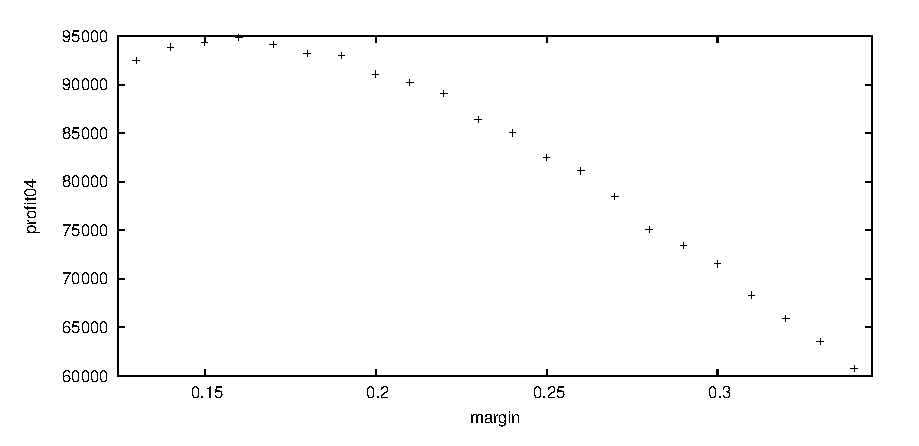
\includegraphics[width=0.8\textwidth]{max-profit-04-f0.eps}\end{center}
  \end{frame}
  \begin{frame}
    \frametitle{Otázky}
    Vysvětlete, proč roste výše optimální marže spolu s růstem velikosti poplatků.\\[1cm]
    Podmínka setrvání:
    \[ \texttt{my-rev} + \texttt{avg-srev-exp} \geq \texttt{be-point} + \texttt{monthly-fee} \]
    růst poklatku $\Rightarrow$ pokles počtu prodejců $\Rightarrow$ pokles obratu i zisku Oriflame $\Rightarrow$ nutnost kompenzace na straně příjmu prodejců zvýšením jejich marže $\Rightarrow$ zvýšení počtu prodejců $\Rightarrow$ zvýšení obratu i zisku
  \end{frame}
  \begin{frame}
    \frametitle{Otázky}
    Vysvětlete, nakolik výsledky optimalizace idealizované sítě použít pro doporučení pro reálný Oriflame. Jaké další úpravy modelu by mohly zajistit vyšší validitu výsledků optimalizace pro Oriflame?\\[1cm]
    \begin{itemize}
    \item Byla by nutná přesná kalibrace parametrů podle skutečné sítě. Tyto údaje mi ale nejsou k dispozici.
    \item Vytvoření rozmanitější sociální sítě, např. řídce spojené shluky reprezentující města i různé společenské vrstvy.
    \item Zavedení více faktorů do rozhodování osob a možnost změny spotřeby dané osoby.
    \end{itemize}
  \end{frame}

      
% etc
\end{document}
